% Asset ID: FA21ProofDivisibilityLanguageSupportTikZ-001
% Source: CCEA FA21-PROOF-LO001 + Phase 1 proof examples
% Related lesson sections:
%   # 8. Core Theory
%   # 9. Visual Asset Integration
%   # 15. Exam Technique Notes
% Purpose:
%   Induction ladder diagram showing base case, inductive hypothesis,
%   inductive step, and conclusion for divisibility proofs.
% Boundary note:
%   This is the CCEA-core proof route. Divisibility notation is used only
%   as support language for mathematical induction.

\documentclass[tikz,border=10pt]{standalone}

\usepackage{amsmath,amssymb}
\usepackage{xcolor}
\usetikzlibrary{arrows.meta, positioning, calc, decorations.pathreplacing}

\definecolor{Canvas}{HTML}{FAF9F6}
\definecolor{SoftCanvas}{HTML}{FFFFF0}
\definecolor{LineSoft}{HTML}{E5E5EA}
\definecolor{Gold}{HTML}{D4AF37}
\definecolor{GoldDark}{HTML}{C5A059}
\definecolor{TextInk}{HTML}{2C2C2E}
\definecolor{Blush}{HTML}{FBEFEF}

\begin{document}

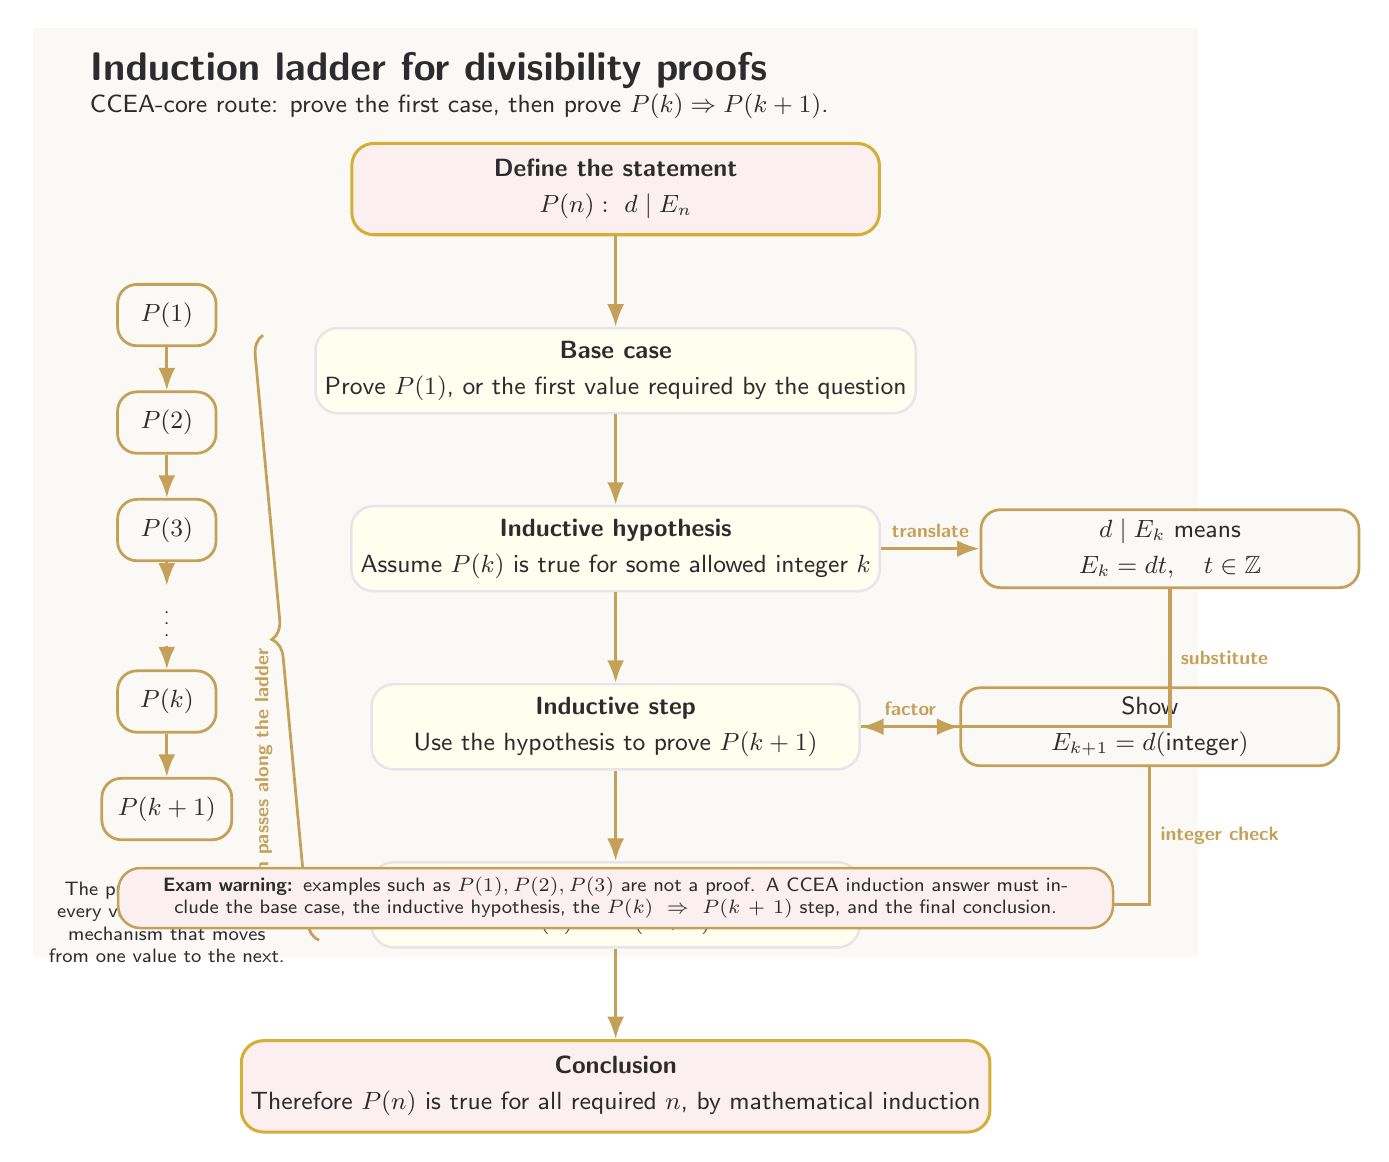
\begin{tikzpicture}[
    x=1cm,
    y=1cm,
    font=\sffamily,
    >=Latex,
    node distance=1.15cm,
    every node/.style={text=TextInk},
    title/.style={font=\sffamily\bfseries\Large, align=left, text=TextInk},
    subtitle/.style={font=\sffamily\small, align=left, text=TextInk},
    stepbox/.style={draw=LineSoft, fill=SoftCanvas, line width=0.9pt, rounded corners=8pt, minimum width=6.2cm, minimum height=1.08cm, align=center, font=\sffamily\small},
    corebox/.style={draw=Gold, fill=Blush, line width=1.1pt, rounded corners=8pt, minimum width=6.7cm, minimum height=1.16cm, align=center, font=\sffamily\small},
    proofbox/.style={draw=GoldDark, fill=Canvas, line width=1pt, rounded corners=7pt, minimum width=4.8cm, minimum height=0.92cm, align=center, font=\sffamily\small},
    arrowline/.style={->, draw=GoldDark, line width=1.15pt},
    label/.style={font=\sffamily\bfseries\scriptsize, text=GoldDark, align=center},
    note/.style={font=\sffamily\scriptsize, align=center, text=TextInk}
]

\fill[Canvas] (-7.4,-9.4) rectangle (7.4,2.4);

\node[title, anchor=west] at (-6.8,1.85) {Induction ladder for divisibility proofs};
\node[subtitle, anchor=west] at (-6.8,1.40)
{CCEA-core route: prove the first case, then prove \(P(k)\Rightarrow P(k+1)\).};

\node[corebox] (define) at (0,0.35)
{\textbf{Define the statement}\\[2pt]
\(P(n):\ d\mid E_n\)};

\node[stepbox, below=of define] (base)
{\textbf{Base case}\\[2pt]
Prove \(P(1)\), or the first value required by the question};

\node[stepbox, below=of base] (hyp)
{\textbf{Inductive hypothesis}\\[2pt]
Assume \(P(k)\) is true for some allowed integer \(k\)};

\node[proofbox, right=1.25cm of hyp] (translate)
{\(d\mid E_k\) means\\[2pt]
\(E_k=dt,\quad t\in\mathbb Z\)};

\node[stepbox, below=of hyp] (step)
{\textbf{Inductive step}\\[2pt]
Use the hypothesis to prove \(P(k+1)\)};

\node[proofbox, right=1.25cm of step] (factor)
{Show\\[2pt]
\(E_{k+1}=d(\text{integer})\)};

\node[stepbox, below=of step] (concludeStep)
{\textbf{Link completed}\\[2pt]
\(P(k)\Rightarrow P(k+1)\)};

\node[corebox, below=of concludeStep] (final)
{\textbf{Conclusion}\\[2pt]
Therefore \(P(n)\) is true for all required \(n\), by mathematical induction};

\draw[arrowline] (define) -- (base);
\draw[arrowline] (base) -- (hyp);
\draw[arrowline] (hyp) -- (step);
\draw[arrowline] (step) -- (concludeStep);
\draw[arrowline] (concludeStep) -- (final);
\draw[arrowline] (hyp.east) -- node[label, above] {translate} (translate.west);
\draw[arrowline] (translate.south) |- node[label, near start, right] {substitute} (step.east);
\draw[arrowline] (step.east) -- node[label, above] {factor} (factor.west);
\draw[arrowline] (factor.south) |- node[label, near start, right] {integer check} (concludeStep.east);

\draw[decorate, decoration={brace, amplitude=7pt, mirror}, draw=GoldDark, line width=1pt]
    ($(base.west)+(-0.65,0.45)$) -- ($(concludeStep.west)+(-0.65,-0.45)$)
    node[midway, left=0.35cm, label, rotate=90] {truth passes along the ladder};

\node[proofbox, minimum width=1.25cm, minimum height=0.78cm] (p1) at (-5.7,-1.25) {\(P(1)\)};
\node[proofbox, minimum width=1.25cm, minimum height=0.78cm, below=0.55cm of p1] (p2) {\(P(2)\)};
\node[proofbox, minimum width=1.25cm, minimum height=0.78cm, below=0.55cm of p2] (p3) {\(P(3)\)};
\node[note, below=0.30cm of p3] (dots) {\(\vdots\)};
\node[proofbox, minimum width=1.25cm, minimum height=0.78cm, below=0.30cm of dots] (pk) {\(P(k)\)};
\node[proofbox, minimum width=1.65cm, minimum height=0.78cm, below=0.55cm of pk] (pk1) {\(P(k+1)\)};

\draw[arrowline] (p1) -- (p2);
\draw[arrowline] (p2) -- (p3);
\draw[arrowline] (p3) -- (dots);
\draw[arrowline] (dots) -- (pk);
\draw[arrowline] (pk) -- (pk1);

\node[note, text width=3.3cm, below=0.4cm of pk1]
{The proof does not test every value. It proves the mechanism that moves from one value to the next.};

\node[
    draw=GoldDark,
    fill=Blush,
    rounded corners=8pt,
    line width=0.9pt,
    text width=12.4cm,
    align=center,
    font=\sffamily\scriptsize,
    anchor=south
] at (0,-9.05)
{\textbf{Exam warning:} examples such as \(P(1),P(2),P(3)\) are not a proof. A CCEA induction answer must include the base case, the inductive hypothesis, the \(P(k)\Rightarrow P(k+1)\) step, and the final conclusion.};

\end{tikzpicture}

\end{document}
